%% For double-blind review submission, w/o CCS and ACM Reference (max submission space)
\documentclass[sigplan,review,anonymous]{acmart}\settopmatter{printfolios=true,printccs=false,printacmref=false}
%% For double-blind review submission, w/ CCS and ACM Reference
%\documentclass[sigplan,review,anonymous]{acmart}\settopmatter{printfolios=true}
%% For single-blind review submission, w/o CCS and ACM Reference (max submission space)
%\documentclass[sigplan,review]{acmart}\settopmatter{printfolios=true,printccs=false,printacmref=false}
%% For single-blind review submission, w/ CCS and ACM Reference
%\documentclass[sigplan,review]{acmart}\settopmatter{printfolios=true}
%% For final camera-ready submission, w/ required CCS and ACM Reference
%\documentclass[sigplan]{acmart}\settopmatter{}
\usepackage{amsmath}
\usepackage{xspace}
\definecolor{uwpurple}{RGB}{128,0,128}
\newcommand{\jln}[1]{\textcolor{uwpurple}{\textit{[{#1} --JLN]}}}
\newcommand{\sak}[1]{\textcolor{green}{\textit{[{#1} --SK]}}}
\usepackage{syntax}
%% Conference information
%% Supplied to authors by publisher for camera-ready submission;
%% use defaults for review submission.
\acmConference[PL'18]{ACM SIGPLAN Conference on Programming Languages}{January 01--03, 2018}{New York, NY, USA}
\acmYear{2018}
\acmISBN{} % \acmISBN{978-x-xxxx-xxxx-x/YY/MM}
\acmDOI{} % \acmDOI{10.1145/nnnnnnn.nnnnnnn}
\startPage{1}

%% Macros for quantities
\newcommand{\NumApps}{{\color{red} XX}\xspace}
\newcommand{\NumRulesFixed}{{\color{red} XX}\xspace}
\newcommand{\NumPredicatesRelaxed}{{\color{red} XX}\xspace}
\newcommand{\NumOrderingProblems}{{\color{red} XX}\xspace}
\newcommand{\NumRulesSynthesized}{{\color{red} XX}\xspace}
\newcommand{\NumFailureExamples}{{\color{red} XX}\xspace}



%% Copyright information
%% Supplied to authors (based on authors' rights management selection;
%% see authors.acm.org) by publisher for camera-ready submission;
%% use 'none' for review submission.
\setcopyright{none}
%\setcopyright{acmcopyright}
%\setcopyright{acmlicensed}
%\setcopyright{rightsretained}
%\copyrightyear{2018}           %% If different from \acmYear

%% Bibliography style
\bibliographystyle{ACM-Reference-Format}
%% Citation style
%\citestyle{acmauthoryear}  %% For author/year citations
%\citestyle{acmnumeric}     %% For numeric citations
%\setcitestyle{nosort}      %% With 'acmnumeric', to disable automatic
                            %% sorting of references within a single citation;
                            %% e.g., \cite{Smith99,Carpenter05,Baker12}
                            %% rendered as [14,5,2] rather than [2,5,14].
%\setcitesyle{nocompress}   %% With 'acmnumeric', to disable automatic
                            %% compression of sequential references within a
                            %% single citation;
                            %% e.g., \cite{Baker12,Baker14,Baker16}
                            %% rendered as [2,3,4] rather than [2-4].


%%%%%%%%%%%%%%%%%%%%%%%%%%%%%%%%%%%%%%%%%%%%%%%%%%%%%%%%%%%%%%%%%%%%%%
%% Note: Authors migrating a paper from traditional SIGPLAN
%% proceedings format to PACMPL format must update the
%% '\documentclass' and topmatter commands above; see
%% 'acmart-pacmpl-template.tex'.
%%%%%%%%%%%%%%%%%%%%%%%%%%%%%%%%%%%%%%%%%%%%%%%%%%%%%%%%%%%%%%%%%%%%%%


%% Some recommended packages.
\usepackage{booktabs}   %% For formal tables:
                        %% http://ctan.org/pkg/booktabs
\usepackage{subcaption} %% For complex figures with subfigures/subcaptions
                        %% http://ctan.org/pkg/subcaption


\begin{document}

%% Title information
\title{Automatically improving Halide’s simplifier with synthesis}         %% [Short Title] is optional;
                                        %% when present, will be used in
                                        %% header instead of Full Title.
\titlenote{with title note}             %% \titlenote is optional;
                                        %% can be repeated if necessary;
                                        %% contents suppressed with 'anonymous'
\subtitle{Subtitle}                     %% \subtitle is optional
\subtitlenote{with subtitle note}       %% \subtitlenote is optional;
                                        %% can be repeated if necessary;
                                        %% contents suppressed with 'anonymous'


%% Author information
%% Contents and number of authors suppressed with 'anonymous'.
%% Each author should be introduced by \author, followed by
%% \authornote (optional), \orcid (optional), \affiliation, and
%% \email.
%% An author may have multiple affiliations and/or emails; repeat the
%% appropriate command.
%% Many elements are not rendered, but should be provided for metadata
%% extraction tools.

%% Author with single affiliation.
\author{First1 Last1}
\authornote{with author1 note}          %% \authornote is optional;
                                        %% can be repeated if necessary
\orcid{nnnn-nnnn-nnnn-nnnn}             %% \orcid is optional
\affiliation{
  \position{Position1}
  \department{Department1}              %% \department is recommended
  \institution{Institution1}            %% \institution is required
  \streetaddress{Street1 Address1}
  \city{City1}
  \state{State1}
  \postcode{Post-Code1}
  \country{Country1}                    %% \country is recommended
}
\email{first1.last1@inst1.edu}          %% \email is recommended

%% Author with two affiliations and emails.
\author{First2 Last2}
\authornote{with author2 note}          %% \authornote is optional;
                                        %% can be repeated if necessary
\orcid{nnnn-nnnn-nnnn-nnnn}             %% \orcid is optional
\affiliation{
  \position{Position2a}
  \department{Department2a}             %% \department is recommended
  \institution{Institution2a}           %% \institution is required
  \streetaddress{Street2a Address2a}
  \city{City2a}
  \state{State2a}
  \postcode{Post-Code2a}
  \country{Country2a}                   %% \country is recommended
}
\email{first2.last2@inst2a.com}         %% \email is recommended
\affiliation{
  \position{Position2b}
  \department{Department2b}             %% \department is recommended
  \institution{Institution2b}           %% \institution is required
  \streetaddress{Street3b Address2b}
  \city{City2b}
  \state{State2b}
  \postcode{Post-Code2b}
  \country{Country2b}                   %% \country is recommended
}
\email{first2.last2@inst2b.org}         %% \email is recommended


%% Abstract
%% Note: \begin{abstract}...\end{abstract} environment must come
%% before \maketitle command
\begin{abstract}
  The wide adoption of Halide as an efficient domain-specific language
  for image processing and tensor computation shows the language is
  useful and effective for compiling high performance code across platforms.
  In Halide, reasoning about the code relies on a term rewriting system to
  prove properties required for efficient and correct compilation.  This rewrite
  system is written as a large collection of ad hoc hand-written transformation rules 
  that incrementally rewrite expressions into simpler forms.
  In this work, we apply formal techniques to prove the correctness of existing
  rewrite rules and formalize an ordering that ensures termination.  Then,
  we build an automatic program synthesis system that creates new, provably
  correct rules from failure cases where the compiler was unable to prove properties. We
  identify and fix \NumRulesFixed incorrect rules and \NumOrderingProblems rules
  with ordering that may result in infinite looping. We augment existing rules
  with a system that automatically synthesizes provably-correct new rules from
  failed proof examples, adding \NumRulesSynthesized new rules. We show the new
  term rewriting system is more correct, more robust, and more general,
  and enables faster performance for generated code.
\end{abstract}


%% 2012 ACM Computing Classification System (CSS) concepts
%% Generate at 'http://dl.acm.org/ccs/ccs.cfm'.
\begin{CCSXML}
<ccs2012>
<concept>
<concept_id>10011007.10011006.10011008</concept_id>
<concept_desc>Software and its engineering~General programming languages</concept_desc>
<concept_significance>500</concept_significance>
</concept>
<concept>
<concept_id>10003456.10003457.10003521.10003525</concept_id>
<concept_desc>Social and professional topics~History of programming languages</concept_desc>
<concept_significance>300</concept_significance>
</concept>
</ccs2012>
\end{CCSXML}

\ccsdesc[500]{Software and its engineering~General programming languages}
\ccsdesc[300]{Social and professional topics~History of programming languages}
%% End of generated code


%% Keywords
%% comma separated list
\keywords{keyword1, keyword2, keyword3}  %% \keywords are mandatory in final camera-ready submission


%% \maketitle
%% Note: \maketitle command must come after title commands, author
%% commands, abstract environment, Computing Classification System
%% environment and commands, and keywords command.
\maketitle


\section{Introduction}
Tensor and image processing pipelines power a large number of applications,
including computational photography, medical imaging, machine learning,
and computer vision, which run on a large variety of platforms, from
mobile phones to large-scale servers in the cloud.  For many of these
applications, high performance is an essential requirement due to real-time
requirements, compute cost, and battery life.

Halide~\cite{siggraph2012jrk, pldi2013jrk} has proven to be an effective
domain-specific language (DSL) for writing such code and obtaining cross-platform
high performance, with multiple industrial vendors relying on Halide to power
applications used by millions of users on mobile phones, tablets, desktops, and
servers.  Halide separates what is computed (the \textit{algorithm}) from how
the computation executes (the \textit{schedule}); the compiler ensures that
different schedules for different platforms correctly compute the algorithm.
Schedules often require the compiler to prove specific properties in order
to guarantee correctness or to ensure the resulting code performs as well
as possible.  For example, to fully unroll a loop, the compiler must prove
the loop has a constant extent.

Many of these properties relate regions of computation with one another,
which, within Halide, are represented as intervals over the integers.
Reasoning about these regions uses a \textit{term rewriting system}
(TRS) on integers: the compiler applies simplification rules to an expression relating
the regions until no more rewrites apply.  The final expression can be
true, false, or indeterminate.  Indeterminate values may prevent optimizations
from being applied, resulting in errors during compilation, or may result
in the compiler producing suboptimal code.

The Halide TRS must balance compilation speed and applicability.  For the widest applicability,
a TRS must be \textit{convergent}, meaning that if two expressions are equal, then the TRS
will always produce the same final canonical form.  However, constructing a TRS of this form
is \sak{impossible? inefficient?}.  In Halide's compiler, the TRS consists of a series of
hand-written rules and efficient matchers to match rules bottom-up.  These rules were constructed
by developers based on observed compilation failures over many years, and ordered in ad-hoc ways
to avoid non-termination.  Extensive fuzz-testing has been able to find bugs in rewrite rules,
but there is no guarantee bugs do not continue to persist.  Furthermore, adding additional
rules requires expert programmers to meticulously analyze compilation failures and hand-craft
rules that mitigate the problems without causing new errors.

In this work, we improve the Halide term rewriting system by  formally checking the existing
set of rules to ensure correctness, and then further constructing a rule ordering that 
ensures termination.  We then automate the task of writing new rules by building a program
synthesis system that automatically checks compilation failures for expressions that are
correct but not provable, produces new rules, predicates to guard their application, and
a placement within the rule ordering to prevent non-termination.

The verification and synthesis
of these rules poses significant challenges: the underlying theory of non-linear integer arithmetic (NLIA)
is known to be undecidable.  We verify existing rules using a combination of the Z3~\cite{de2008z3} satisfiability
modulo theory (SMT) solver, the Coq~\cite{coq19} interactive theorem prover, and a hand-written solver
that uses beam search with a learned cost model.  New rules are constructed with Z3 (for linear rules)
and the new solver.  To search for cases where the Halide compiler fails to prove properties, we run
\NumApps existing Halide pipelines with randomized schedules, and augment this set with a random pipeline
generator designed to produce plausible image processing and machine learning pipelines.

Overall, we discover \NumRulesFixed bugs in hand-written Halide simplifier rules, and discover \NumOrderingProblems
potential issues in rule ordering.  We then synthesize \NumRulesSynthesized new rules from \NumFailureExamples and
demonstrate that our approach reduces compilation failures, does not slow down the compiler, and improves
the performance of generated code.

\subsection{Why this and not some other thing?}
\jln{These are just notes}
\subsubsection{Why not use z3 for simplification?}

Z3 tends to be very fast for many cases and bog down in a minority of cases. The Halide algorithm has a smoother performance curve. 

Z3 is general-purpose, but we need not be. The handwritten simplifier ruleset was written to address expressions that are generated by the Halide compiler. Since we are driven by a subset of all Halide expressions and not arbitrary expressions in the Halide expression language, we can specialize and in some cases solve expressions that Z3 cannot. 

The Halide simplifier must be deterministic. Even with a fixed random seed, Z3 is not complete for NLIA and may time out on difficult queries, thus it's possible that one run will find a solution when another will not.

\subsubsection{Why not use an egraph/other TRS algorithm for simplification?}

\jln{as mentioned above, it would be nice to state here that a confluent TRS for NLIA is impossible}

Egraphs are memory-intensive while the Halide TRS is not.

Egraphs grow their equivalence classes with each invocation of their rulesets until they converge or until their graph grows so large that progress is no longer possible. Since we can't guarantee that our rules converge, the problem is reaching the goal state before the growth of the graph reaches that infeasible inflection point.

Egraph handling of predicates is also more computationally expensive than the Halide TRS; Halide evaluates constants at compile time to see if a predicate obtains on a particular expression. Since egraphs have no knowledge of semantics, the machinary for handling predicates is much more involved.

If bounded, egraphs are also deterministic, so that's not a problem.

I know that dumping the Halide ruleset into an egraph is completely unworkable, since I tried it -- not a fair comparsion since you would tune an egraph's ruleset differently.

The Halide TRS gives a nice starting point for synthesis because a failed call to the simplifier yields an expression the simplifier can make no progress on. A failed egraph call gives an equivalence class that should include the goal state but doesn't, so it's not as clear how to debug that.


\section{Background}
\subsection{Term Rewriting Systems}
Term rewriting systems~\cite{gorn1967} successively apply \textit{rewrite rules} to transform a given
expression into a simpler form, until no further simplifications are possible.  Such systems are widely
used in theorem proving~\cite{} and abstract interpretation~\cite{}.

Terms are defined inductively over a set of variables $V$ and a set of function symbols $\Sigma$. Every variable $v \in V$ is a term, and for any function symbol $f \in \Sigma$ with arity $n$ and any terms $t_1, ..., t_n$, the application of the symbol to the terms $f(t_1, ..., t_n)$ is also a term. We refer to the set of terms constructed from the variables $V$ and the function symbols $\Sigma$ as $T(\Sigma, V)$.

A \emph{rewrite rule} is a directed binary relation $l \rightarrow r$ such that $l$ is not a variable, and all variables present in $r$ are also present in $l$ (i.e., $\mathcal{V}ar(l) \supseteq \mathcal{V}ar(r)$). A set of rewrite rules is a \emph{term rewriting system}.

Consider a set of terms $T(\Sigma, V)$ such that $\Sigma = \{\otimes, \oplus\}$ and $V$ be an infinite set of variables. Let the term rewriting system $R$ consist of a single rule:

\[ R = \{ x_1 \otimes x_2 \rightarrow x_1 \oplus x_2 \} \]

We use $R$ to rewrite the term

\[ 
(y_1 \oplus y_1) \otimes (y_2 \otimes y_3)
\]

The first step is matching; we find a substitution that will unify the lefthand side (LHS) of the rule with the term we are rewriting. Here, the substitution is:

\[
\{ x_1 \mapsto (y_1 \oplus y_1), x_2 \mapsto (y_2 \otimes y_3) \}
\]

We then apply this substitution to the righthand side (RHS) of the rule to obtain the rewritten version of the original term.

\[ 
(y_1 \oplus y_1) \oplus (y_2 \otimes y_3)
\]

\subsection{Term Rewriting in Halide}

The Halide compiler contains a term rewriting system, currently comprised of
several hundred rules, that operates over the space of Halide
expressions\footnote{See Appendix ~\ref{ss:appendixA} for the full Halide
  expression grammar}. While the term rewriting system is used for multiple
purposes within the compiler, for the purposes of this work the most important
usage is when this TRS serves proof engine to determine if
some equality or inequality holds, or when the rewriter attempts to find tight
bounds on regions. For example, in order to parallelize a
reduction variable, the compiler must prove that there are no hazards, which is
done by using the TRS as proof engine.  Another example is that Halide uses
the TRS to decide how much memory to allocate for intermediates; tighter, more
simplified bounds result in more efficient execution since they eliminate over-allocation.
More generally, proof engine failures can lead to:
\begin{itemize}
\item Insufficiently tight bounds on loops and allocations, which may result in
  runtime failures (e.g. due to memory overallocation) or performance issues;

\item Failure of the compiler to apply optimizations, also resulting in slow performance;

\item Dynamic checks in the generated code, for properties that could have been proven
  at compile time, leading to slower code;

\item Compilation failures, when the compiler is unable to correctly produce code
  even though the properties required hold, or when the proof engine itself crashes
  or loops infinitely.
\end{itemize}
Thus, correctness and generality are essential to make the compiler robust and
able to generate fast code.

%% The compiler also frequently needs to \emph{simplify} Halide expressions.
%% For example, canceling correlated subexpressions aids in proving monotonicity in
%% sliding window optimizations; finding a tight bound on loops or memory
%% allocations is often made possible when expressions have been simplified.
%% \jln{this is handwave-y, fix later} For this reason, we often refer to the
%% Halide term rewriting system as a simplifier.

The design of the term rewriting algorithm has two additional important
requirements. The first is performance: although the simplifier is called at
compile time, it may be invoked hundreds of times in compiling a single pipeline
\jln{is this true?}. Thus, unlike many term rewriting algorithms, the Halide TRS
never backtracks. The second requirement is determinisim: the compiler must
always return the same schedule every time it encounters a particular pipeline.
This precludes any non-deterministic search strategy for the best sequence of
rules to apply, or directly invoking a solver such as Z3, since even with a
fixed random seed machines with different computational power may return
different results within a given timeout.

The Halide term rewriting algorithm simplifies an input expression in a depth-first, bottom-up traversal of the expression DAG. At each node, it looks up the list of rewrite rules that correspond to the node's function symbol, then attempts to match the subtree expression with the rule LHSs in order. When a match is found, it rewrites the subtree expression using the RHS of that rule, and then attempts to simplify the subtree expression again. If no rule matches the subtree, the traversal continues; when the entire expression cannot be simplified further, the rewritten expression is returned. \jln{use example from slides here; also confirm big O performance of this algo}

Halide rewrite rules optionally contain a predicate that must hold for a rule to be applied. Halide expressions may contain constants whose values are known at compile time. Predicate expressions may contain only such constants; when the LHS of a rule matches an expression, its predicate is evaluated and only if it is true will the rewrite be applied. \jln{maybe cite a common case where we know a constant, like a loop bound?}

We limit ourselves to expressions over the set of infinite precision integers in
this work, although Halide expressions can contain floats and fixed-width
integers. However, the uses of the TRS we consider in this work all operate
on infinite integers.

\subsection{Program Synthesis}
Over the past decade, syntax-guided synthesis (SyGuS)~\cite{sygus} has been used
to search over a space of possible programs in order to find one that meets
a semantic specification.  One of the most popular techniques is counterexample-guided
inductive synthesis (CEGIS), which leverages the power of satisfiability modulo theories
(SMT) and SAT solvers to make search over a large space of programs more intelligent.
In CEGIS, the task is to find some program in the search space such that for all possible
inputs, the found program fulfills some semantic criteria, usually equivalence with
a specification.

The CEGIS process proceeds in a loop. Given a specification $S$ and arbitrary
settings for $C = {c_0,..c_i}$, constructing a query to the SMT engine that searches for
a counterexample to equivalence:
$$\forall B, \neg (f(C, B) = S(B))$$
The solver either returns unsatisfiable, meaning the the choices encoded in $C$
indeed result in a program equivalent to $S$, or returns a counter example input $e_0$
for which the two programs give different results.  Then, the CEGIS system constructs a new query,
asking the SMT solver for choices $C'$ such that the two programs are equivalent.
Given the $C'$ returned by the solver, CEGIS then attempts the original query once again.
If a counterexample $e_1$ is found, another iteration of the CEGIS loop begins, this time querying
the solver for $C'$ that results in equivalent behavior to $S$ for both counterexample inputs.
In this manner, the CEGIS loop iterates between querying the solver for new $C'$ valid
for all found counterexamples so far, then queries the SMT solver to prove the new $C'$ is
correct for all inputs.  The loop terminates when the final $C'$ is proven correct for
possible inputs.

\section{Improving Soundness}
\jln{We haven't synthesized any vector op rules; not sure if that's a conscious decision or we haven't really had any in input expressions.}


\subsection{Rule verification}

First, we assure soundness by verifying the current set of handwritten rules. We do this by modeling Halide expressions in SMT2 and sending them to the SMT solver Z3~\cite{de2008z3}. Most of the Halide expression semantics maps cleanly onto SMT2 formulas. The functions \texttt{max} and \texttt{min} are defined in the usual way, and \texttt{select} has the same meaning as the SMT2 operator \texttt{ite}. Division and modulo are given the Euclidean definitions in both Halide and SMT2. If a variable appears in the LHS of a rule as a divisor in a division or modulo operation, it is assumed to be non-zero. The Halide expressions do not have a true boolean type (true and false are represented by unsigned integers of 1 bitwidth), so expressions must be typed as either \texttt{Int} or \texttt{Bool} when translated into SMT2. The Halide expression grammar contains two vector operators, \texttt{broadcast} and \texttt{ramp}; all other integer operators can be coerced to vector operators. The operation \texttt{broadcast} projects some value $x$ to a vector of length $l$; because of the type coercion, we can simply represent \texttt{broadcast(x)} as the variable \texttt{x} in SMT2. The \texttt{ramp} operator creates a vector of length $l$ whose initial entry has the value $x$ and all subsequent entries increase with stride $s$. In SMT2, we represent this term as the symbolic expression $x + l * s$, where $l$ must be zero or positive.

Given this modeling, for each rule, we assert any assumptions are true, then assert that the rule's LHS is not equivalent to its RHS and ask Z3 to find a counterexample. If no counterexample can be found, the LHS must be equivalent to the RHS and the rule must be correct. We implemented a SMT2 printer for the Halide rewrite rules and ran them through Z3; out of 999 rules, we were able to verify 872 as correct and discover 4 incorrect rules; these rules are listed in Table~\ref{tab:incorrectrules}. Rule verification using Z3 is automated and can be run for the current set of rewrite rules via script.

However, nonlinear integer arithmetic is generally undecidable, and for 123 rules, Z3 either timed out or returned unknown. Nearly all of these rules used either division or modulo. We used the proof assistant Coq to manually prove or disprove the correctness of these remaining rules. \jln{about 20 left to go} We were also able to relax the predicates of \jln{TK} rules; for example, a rule with a predicate requiring some constant to be positive would be equally valid if the constant was non-zero.

We also want to guarantee that if an input expression have well-defined behavior, the simplifier will never rewrite it into an expression that has undefined behavior. If an input expression never divides by zero, then the simplifier output should be guaranteed to never divide by zero. We check this by verifying that all terms that are used as divisors or moduluses in the RHS of a rewrite rule also appear as a divisor in the rule's LHS. (Note that all divisor terms on the LHS side are not required to appear in the RHS; if a divisor is factored out, then it is possible that the input expression would have caused a divide-by-zero fault but the simplified expression will not.) \jln{talk about overflow here}

\begin{table*}

\caption{Incorrect rules found during verification.}
\begin{tabular}{|l|l|}
\hline
Incorrect rule & Tool used \\
\hline
$((x + c0)/c1)*c1 - x \rightarrow_R x \bmod c1 \textrm{ if } c1 > 0 \wedge c0 + 1 == c1$ & Z3 \\
$x - ((x + c0)/c1)*c1 \rightarrow_R -(x \bmod c1) \textrm{ if } c1 > 0 \wedge c0 + 1 == c1$ & Z3 \\
$min(x, c0) < min(x, c1) + c2 \rightarrow_R \textrm{false if } c0 >= c1 + c2)$ & Z3 \\
$max(x, c0) < max(x, c1) + c2 \rightarrow_R \textrm{false if } c0 >= c1 + c2$ & Z3 \\
\hline
\end{tabular}
\label{tab:incorrectrules}
\end{table*}

\subsection{Termination}

\jln{note that the ``strength'' of operators is arbitrary for the purposes of proving termination, but meaningful in terms of simplifying (rather than proving) expressions.}

Term rewriting systems are not guaranteed to terminate. Consider a term rewriting system containing only one rule: $x + y \rightarrow y + x$. The term $3 + 5$ matches the LHS of the rule and is rewritten to $5 + 3$, which can again be matched to the rule and rewritten to $3 + 5$, and so on. To guarantee termination irrespective of the rule application algorithm, every application of a rule needs to strictly (monotonically) decrease in some measure. In other words, if $s \rightarrow_R t$, $s > t$ for some strict order $>$. However, since the set of terms is infinite, we cannot check that $s > t$ for all pairs of terms $s, t$. Instead, we show that for every rule $l \rightarrow r$ in our term rewriting system, $l > r$. This will suffice if $>$ is a \emph{reduction order}, given:

\begin{theorem}\label{theorem:terminates}
A term rewriting system $R$ terminates iff there exists a reduction order $>$ that satisfies $l > r$ for all $l \rightarrow r \in R$.
\end{theorem}

Per Baader and Nipkow~\cite{baader1999term}, a reduction order is defined as follows.

\begin{definition}
A strict order on terms $T(\Sigma, V)$ is a reduction order iff: 
\begin{enumerate}
    \item well-founded, or terminating,
    \item compatible with $\Sigma$-operations: for all $s_1, s_2 \in T(\Sigma,V)$, all $n \geq 0$, and all $f \in \Sigma^{(n)}$, $s_1 > s_2$ implies
    \[ f(t_1,...t_{i-1},s_1,t_{i+1},...,t_n) > f(t_1,...t_{i-1},s_2,t_{i+1},...,t_n)
    \]
    for all $i, 1 \leq i \leq n$ and all $t_1,...t_{i-1},t_{i+1},...,t_n \in T(\Sigma,V)$.
    \item closed under substitution: for all $s_1, s_2 \in T(\Sigma,V)$ and all substitutions $\sigma \in \mathcal{S}ub(T(\Sigma,V))$, $s_1 > s_2$ implies $\sigma(s_1) > \sigma(s_2)$.
\end{enumerate}
\end{definition}

We demonstrate our reduction order over a simpler set of terms defined by the function symbol set $\Sigma = \{\oplus, \otimes\}$ and the unbounded set of variables $V = \{x_1, x_2, \ldots \}$. This easily generalizes to the full set of Halide terms.

First, we need to define an order that is well-founded. We do this by defining a measure function that embeds terms into the natural numbers. We define a function $\phi_\otimes$:

\[
\phi_\otimes(s) = \textrm{count of occurrences of } \otimes \textrm{ in the term } s
\]

We can use this measure function to define a strict order $>_\otimes$:

\[
s_1 >_\otimes s_2 \iff \phi_\otimes(s_1) > \phi_\otimes(s_2)
\]

Since $\phi_\otimes$ provides a mapping from terms to the natural numbers, $<_\otimes$ must be well-founded. We can also easily see that $>_\otimes$ is compatible with $\Sigma$-operations.

\[
\begin{aligned}
\phi_\otimes(f(t_1, \ldots, t_{i-1}, s_1, t_{i+1}, \ldots, t_n)) = \\
\phi_\otimes(s_1) + \sum^{t_i} \phi_\otimes(t_i) + \begin{cases} 1 & f = \otimes \\
0 & \textrm{otherwise} \end{cases}
\end{aligned}
\]

Since the summation of the $\phi_\otimes(t_i)$ terms and the piecewise functions are the same for both terms, the property holds.

However, the order is not closed under substitution. Consider:

\[
x_1 \otimes x_2 >_\otimes x_2 \oplus x_2
\]
\[
\sigma(x_2) = x_3 \otimes x_3
\]

Applying the substitution produces more $\otimes$ operations in the righthand term than on the left.

\[
x_1 \otimes (x_3 \otimes x_3) \ngtr_\otimes (x_3 \otimes x_3) \oplus (x_3 \otimes x_3)
\]
 
We must refine the definition of our order. We define a new function $|s|_x$ to denote the number of occurrences of the variable $x$ in the term $s$. Thus, $|x_1 \otimes x_2|_{x_1} = 1$ and $|x_1 \oplus x_1|_{x_1} = 2$. We redefine the order $>_\otimes$ to add the condition that for all variables $x \in V$, the number of occurrences of the variable $x$ in $s_1$ must be equal or greater than the number of occurrences in $s_2$.
\[
s_1 >_\otimes s_2 \iff \phi_\otimes(s_1) > \phi_\otimes(s_2) \wedge \forall x \in V, |s_1|_x \geq |s_2|_x
\]

The redefined order is still well-founded and compatible with $\Sigma$-operations. To show that our redefined order is closed under substitutions via proof by contradiction, let us assume that for some $s, t$, $s >_\otimes t$ and for some substitution $\sigma$, $\sigma(s) \ngtr_\otimes \sigma(t)$. Substitutions can only cause the value of $\phi_\otimes$ to increase. Let $\sigma = \{x_1 \mapsto t_1\}$, and let $s$ be a term that contains the variable $x_1$. If $\phi_\otimes(t_1) = 0$, then $\phi_\otimes(\sigma(s)) = \phi_\otimes(s)$. If $\phi_\otimes(t_1) > 0$, then $\phi_\otimes(\sigma(s)) > \phi_\otimes(s)$. Thus, in order to find some $\sigma$ such that $s >_\otimes t \wedge \sigma(s) \ngtr_\otimes \sigma(t)$, we need to find some $x$ in the term $t$ that increases the count of $\otimes$ operations. But, any such $x$ must occur in $t$ an equal or greater number of times in $s$ and thus must increase the $\phi_\otimes(\sigma(s))$ by an equal or greater value than the increase from $\phi_\otimes(t)$ to $\phi_\otimes(\sigma(t))$. Thus, a contradiction is found and the assertion is proved.


\begin{theorem}
The lexicographic product of two terminating relations is again terminating.
\end{theorem}

Thus, we define an order using a measure function for every $f \in \Sigma$, and then take the lexicographic product of these orders to define a reduction order. Since we evaluate this order by calculating a histogram of operators in each term, we refer to this order as $<_H$. The order in which the function counts are considered lexicographically is given in Appendix~\ref{symbolstrength}. 

Note that while variable elimination is desirable, we cannot use a measure function that counts the number of variable occurrences in a term when composed with the other orders. For example, let $\Sigma = \{\oplus, \otimes\}$ and $V = \{x, y\}$, and let $>_H$ be the lexicographic product of the orders $>_{\oplus}, >_{\otimes}, >_v$. Here $x \otimes x >_H x$, but the order is not closed under substitution. For a substitution $\sigma(x) = y \oplus y$, we have $(y \oplus y) \otimes (y \oplus y) \ngtr y \oplus y$. 

However, we frequently want to normalize terms without changing the number of occurrences of function symbols within them. To permit such rules, we take the lexicographic order of $>_H$ with one more order. The measure function for our last tie-breaking order takes the root symbol of the AST of a term and translate it to a number based on the function count priority as given above. Since we prefer ``stronger'' symbols to be higher in the tree, here the order is reversed. For example, the root symbol of $select(x, y, z) - y$ is $-$ and the root symbol of $select(x, 0, z - y))$; since $-$ is ``weaker'' than $select$, we say $select(x, y, z) - y >_{root} select(x, 0, z - y))$.

\jln{Here we need to either talk about existing rules that don't conform to our reduction order, or figure out how to deal with those rules}



\section{Increasing Completeness: Synthesizing Rewrite Rules}
\begin{figure}
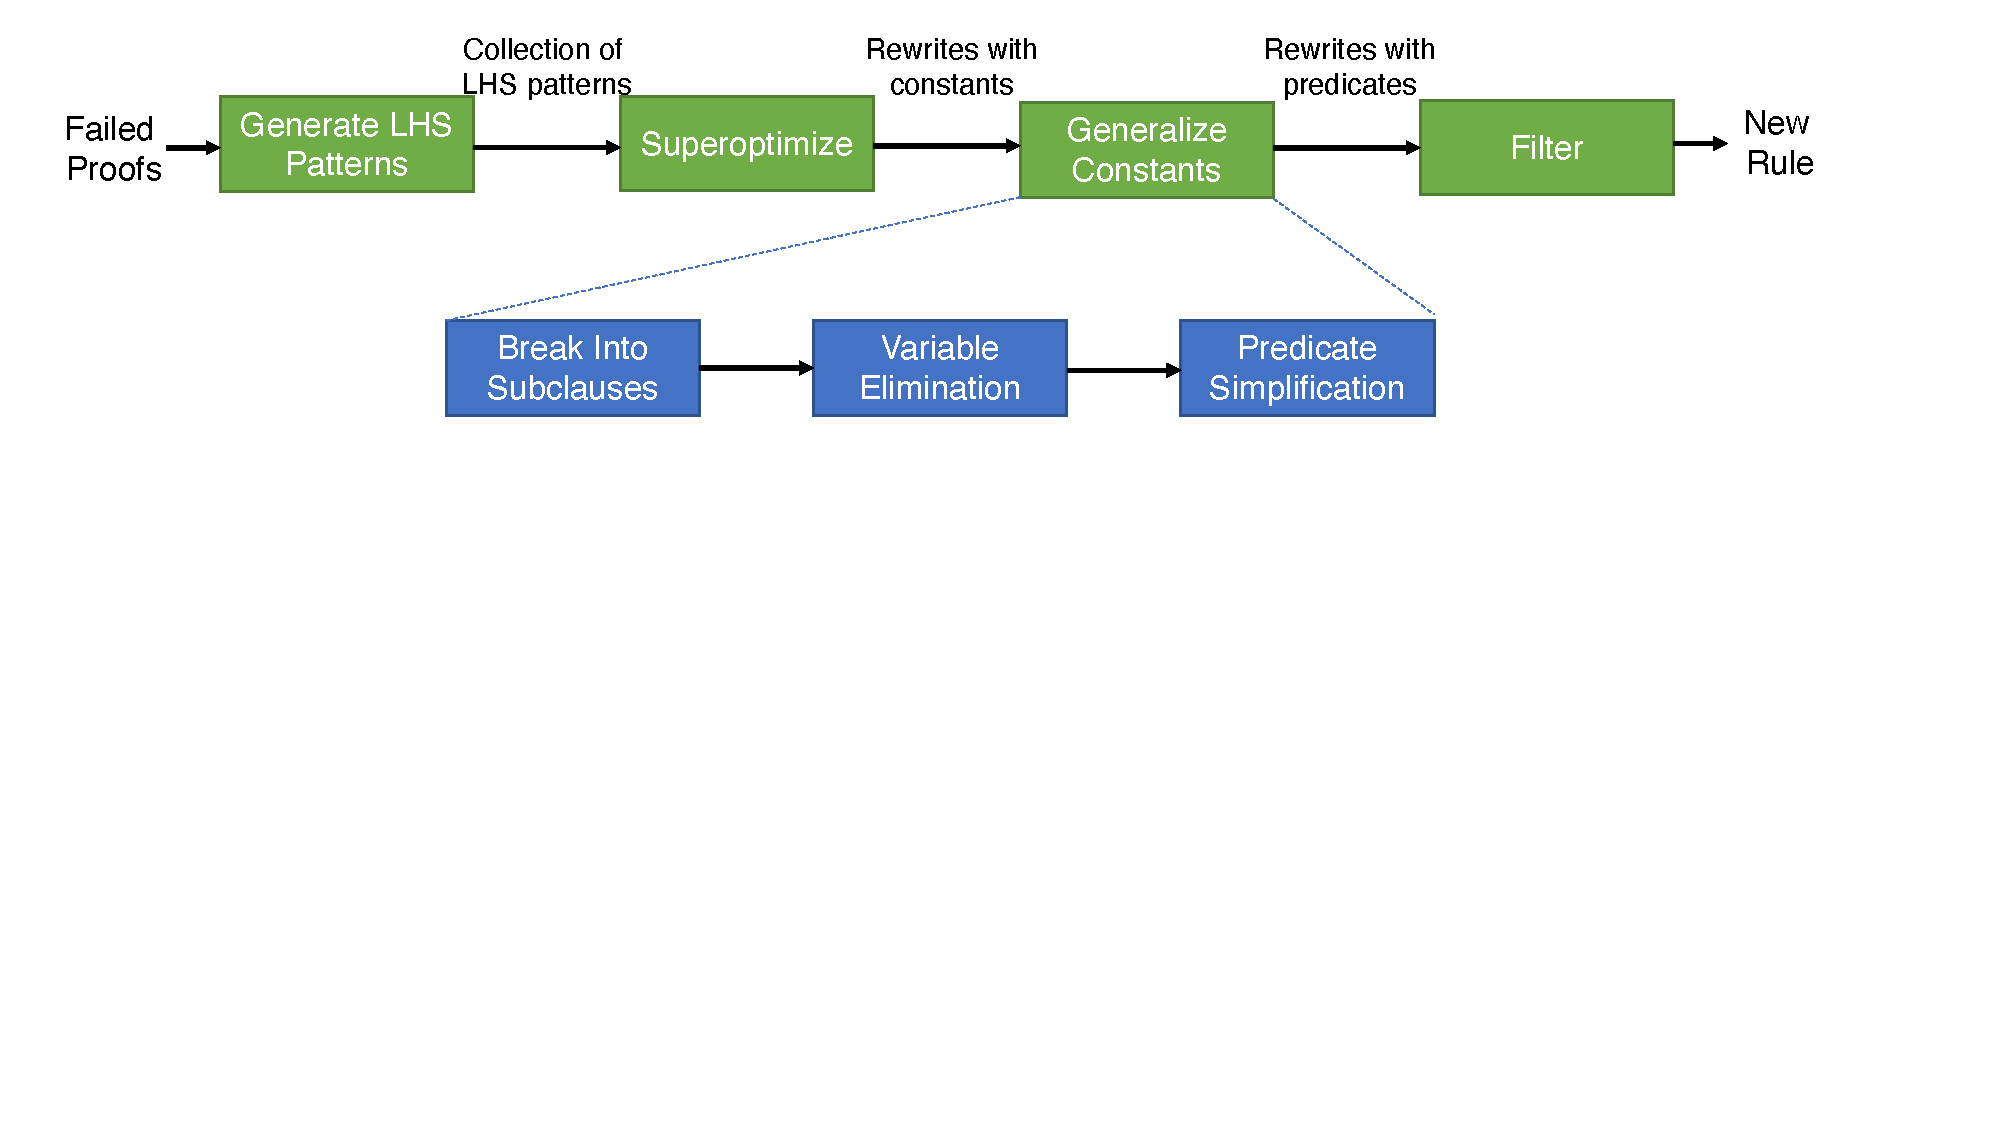
\includegraphics[width=\columnwidth]{figures/synthesis-flow.pdf}
\caption{Overall flow of the synthesis pipeline.}
\label{fig:synthesis-flow}
\end{figure}


The Halide term rewriting system is not complete, by which we mean that there exist expressions checked by the compiler running on real-world pipelines that the simplifier cannot resolve, but which are known to be true. \jln{there should be more discussion of TRS properties here (confluence etc) and whether they are decidable for the Halide lang} We propose a workflow to augment the simplifier using synthesis.

\subsection{Synthesizing candidate rules}

We begin synthesis with a Halide expression we would like to simplify further, but on which the existing simplifier can make no further progress. First, we build a set of potential LHS expressions. We parse the expression as an AST, and find all possible substitutions over the expression by choosing a fresh variable for each subtree. For every possible combination of these substitutions, we perform the substitutions on the original expression, take every subtree of the resulting expression, rename the variables for consistency, and add them to our set of potential LHS patterns. When this is done, we have every possible LHS pattern that could match the original expression. This is exponential in the size of the original expression, but because many of the resulting expressions are redundant, because many combinations of substitutions are incompatible with each other, and because the size of the original expressions tends to be not too large, the resulting set is tractable. We limit the LHS patterns to contain no more than six unique variables. We also remove patterns that contain no repeated variables, since these are unlikely to yield any new rules.

We choose one of our potential LHS expressions and attempt to synthesize a RHS expression. To be a viable candidate rule, we need the RHS to be equivalent to the LHS, and for our reduction order to hold over the expressions such that $LHS <_R RHS$. We synthesize these expressions using a CEGIS loop.

We synthesize a RHS pattern by creating a program sketch and asking the solver Z3 to complete it. The program sketch is made up a list of registers; each register holds an op code, representing an operation from the Halide grammar, and two integers representing arguments to that operation. Those integers may represent indexes to previous registers, or to integer constants. We initialize with a sketch completed by all zeroes to give us a first candidate program. We then enter the CEGIS loop; we posit that the LHS pattern and the candidate RHS are equivalent and ask for a counterexample assignment to their variables that would disprove this assertion. We first try random inputs for reasons of efficiency; if this does not yield any counterexamples, we call out to the solver, and if it cannot find any counterexamples, we know the two expressions must be equivalent and we have a candidate rule. If we do find a counterexample, we add it to our list of counterexamples and ask the solver for a new completion of the sketch such that the completed sketch is equivalent to the LHS pattern for all counterexample variable assignments. We begin with a program sketch of 1 instruction; if no equivalent program of that size is found, we increase the program length by one and start the CEGIS loop again. We stop our search after failing to synthesize a RHS of equivalent length to the original LHS expression.

Once we have produced a candidate rule, we check that it obeys our reduction order ($LHS <_R RHS$) and that all divisor terms in the RHS appear as divisors on the LHS. If either of these properties is violated, we discard the rule. For performance reasons we do not encode these properties into the CEGIS synthesis queries. Our choice to synthesize RHS terms that contain as few operations as possible serves as an approximation of the histogram counts that make up the first of the composed reduction orders. In practice, few synthesized rules are found that violate the reduction order.

The Halide expressions we use as inputs frequently contain integer constants. These constants often occur as coefficients or divisors, and leaving them in place, rather than replacing them with fresh variables, greatly accelerates synthesis of RHS expressions (in many cases replacing constants with variables would leave Z3 able to make no progress in synthesis at all). However, if our candidate rule contains constants, it is unlikely to frequently match to other expressions and thus is overfitted to the input expression. To combat this problem, we generalize constants to fresh variables and where necessary, synthesize predicates to ensure the rule's validity.

\subsection{Synthesizing rule predicates}

Given a candidate rule whose LHS and RHS contain constants, we replace each constant with a fresh \emph{constant variable}. A constant variable can only match against a constant; in other words, against a term whose value is known at compile time. We first query Z3 again to see if the equivalence still holds; if it does, the rule is valid without a predicate. If it is not, we will need to find a predicate to guard applications of the rule in the simplifier. We attempt to synthesize a predicate such that $pred \rightarrow LHS = RHS$ and all the variables that appear in the predicate are constant variables.

Consider the synthesized rule $c0 \cdot x > c1 \cdot x = x > c2$, where $c0, c1, c2$ are constant variables. We want to find some term $t_p$ such that $t_p \rightarrow c0 \cdot x > c1 \cdot x = x > c2$ and $\mathcal{V}ar(t_p) \subseteq \{c0, c1, c2\}$. For some rule $R$, we begin by negating $R$ and deriving as many facts from it as possible that refer only to the constant variables. Once we have found $\not R \rightarrow \not P$, we know that $P \rightarrow R$.


\section{Evaluation}
In this section, we describe experiments to evaluate the improvements made to the Halide term rewriting system.  Specifically, we
test the following hypotheses:
\begin{enumerate}
\item Our improvements to the Halide TRS increases the robustness of the compiler and reduces compilation failures.
\item The improved TRS is more correct.
\item This improved robustness and correctness does not come at the cost of vastly slower compilation speed.
\item Improving the TRS increases performance of generated code.
\end{enumerate}

We perform all experiments on (Andrew's machine: i9-9960X CPU @ 3.10GHz, Ubuntu 18.04, 16 threads using avx-512, LLVM 8.0.1).

\subsection{Robustness}

Our hypothesis is that adding the newly synthesized rules to the Halide simplifier has increased the set of expressions it can simplify. Since the simplifier is non-confluent both before and after the new rules were added, we have no theoretical guarantee that this is the case (in fact, it is possible that the augmented simplifier might fail to simplify an expression that would previously have succeeded if the new rules move the expression into a local minimum). We test the robustness of the enhanced simplifier empirically by compiling randomly generated schedules with the original and enhanced simplifier and reporting the number of compilation failures.

% could also report calls to can_prove and successful calls to can_prove; this is more meaningful as a ratio

\subsection{Correctness}

As described above, we improved the correctness of the simplifier by verifying the existing rules using a combination of Z3 and Coq. We found \NumRulesFixed incorrect rules and submitted patches to the Halide developers. We also found \NumPredicatesRelaxed rules whose predicates could be relaxed while retaining correctness.

\jln{Is it possible that the incorrect rules ever led to unsound compilation output? Not sure how to determine this.}

We also ensure the termination of the simplifier by devising a reduction order over its rewrite rules. We identify \NumOrderingProblems rewrite rules that do not conform to this ordering. 

\subsection{Compilation Speed}

We hypothesize that the Halide simplifier scales well in terms of the number of rewrite rules it uses, and thus adding synthesized rules will not greatly affect compilation times. We need empirical results to confirm this hypothesis, since adding rewrite rules could potentially improve simplification time for one expression and degrade it for another. If no rules match a given expression, the simplifier must try to match every applicable rule, so adding rules would increase simplification time; if a new rule allows the simplifier to make progress on a previously unsimplifiable rule, the simplifier will be able to continue working on the expression and thus take more steps. On the other hand, a new rule might allow an expression to simplify to a small expression quickly, thus reducing the number of rewrite steps the simplifier must take; furthermore, if the simplifier can now successfully prove a term when it could not before, it may be able to use some optimization, thus shortening (non-simplifier) compilation time overall.

We recorded the compilation times for the random schedules used in the robustness experiment above.

\jln{Ras suggests we record can\_prove expressions and get timing on simplifying them so we can separate simplifier timing from the full compliation times.}

\subsection{Generated Code Performance}

By increasing the robustness of the simplifier, we hypothesize that we increase the likelihood that the compiler will return more performant code. Halide ships with X sample applications; we compiled these applications with and without the newly synthesized rules and measured their runtime performance.

% metrics, discussion of results here


\section{Related Work}

Program synthesis has been applied to term rewriting systems in Swapper~\cite{singh2016swapper}, a tool that learns a set of rewrite formulas to transform SMT formulas into forms that can be more easily solved by theory solvers. Swapper takes a training set of formulas drawn from a target domain, does probabilistic sampling to choose LHS candidates, synthesizes predicates and RHS, and finally autotunes the resulting ruleset to choose a rule subset and rule order that gives the best solver performance. Unlike our work, Swapper is an optimizer rather than a prover. Because our rewrite algorithm scales well in terms of the number of rules, we simply use all candidate LHS terms for synthesis rather than sampling. Swapper synthesizes RHS terms that have fewer AST nodes than their corresponding LHS terms; this is not a reduction order and does not guarantee termination, although the autotuning step should reject rulesets with cycles. Finally, Swapper creates a fresh term rewriting system with each invocation, whereas our work augments and maintains an existing term rewriting system.

Butler et al.~\cite{butler2017synthesizing} uses synthesis to learn human-interpretable strategies for puzzle games such as Sudoku or Nonograms. Strategies consist of a pattern (LHS term with variables), condition (predicate), and action (RHS term expressing rewrite), and so comprise a term rewriting system. Strategies are synthesizing Rosette, using a CEGIS loop similar to our synthesis process. Progress in these puzzle games is always monotonic, which gives a natural reduction order. Their goal is to model human strategies, which are greedy and non-deterministic, so they do not consider rule priority or any particular term rewriting algorithm. 

Herbie, superoptimization, abstract interpretation, MCSAT (Jovanovic)

\section{Conclusion}


%% Acknowledgments
\begin{acks}                            %% acks environment is optional
                                        %% contents suppressed with 'anonymous'
  %% Commands \grantsponsor{<sponsorID>}{<name>}{<url>} and
  %% \grantnum[<url>]{<sponsorID>}{<number>} should be used to
  %% acknowledge financial support and will be used by metadata
  %% extraction tools.
  This material is based upon work supported by the
  \grantsponsor{GS100000001}{National Science
    Foundation}{http://dx.doi.org/10.13039/100000001} under Grant
  No.~\grantnum{GS100000001}{nnnnnnn} and Grant
  No.~\grantnum{GS100000001}{mmmmmmm}.  Any opinions, findings, and
  conclusions or recommendations expressed in this material are those
  of the author and do not necessarily reflect the views of the
  National Science Foundation.
\end{acks}


%% Bibliography
\bibliography{bib}


%% Appendix
\appendix
\section{Appendix}

\subsection{Halide expression grammar}
\label{ss:appendixA}

\jln{vector ops are missing}

\begin{grammar}
<Expr> ::= <BoolExpr> 
\alt <IntExpr> 
\alt <VectorExpr>

<BoolExpr> ::= `true'
\alt `false'
\alt <IntExpr> `<' <IntExpr>
\alt <IntExpr> `>' <IntExpr>
\alt <IntExpr> `<=' <IntExpr>
\alt <IntExpr> `>=' <IntExpr>
\alt <IntExpr> `=' <IntExpr>
\alt <IntExpr> `!=' <IntExpr>
\alt <BoolExpr> `&&' <BoolExpr>
\alt <BoolExpr> `||' <BoolExpr>
\alt `!' <BoolExpr>

<IntExpr> ::= <IntExpr> `+' <IntExpr>
\alt <IntExpr> `-' <IntExpr>
\alt <IntExpr> `*' <IntExpr>
\alt <IntExpr> `/' <IntExpr>
\alt <IntExpr> `\%' <IntExpr>
\alt `max' <IntExpr> <IntExpr>
\alt `min' <IntExpr> <IntExpr>
\alt `select' <BoolExpr> <IntExpr> <IntExpr>
\alt integers

<VectorExpr> ::= vectors
\end{grammar}

\subsection{Halide reduction orders}

For some term $s \in T(\Sigma, V)$ and some variable $x \in V$, let $|s|_x$ be the number occurrences of the variable $x$ in the term $s$. For each function symbol $f$ in the set of Halide operators:

\[
\phi_f(s) = \textrm{count of occurrences of } f \textrm{ in the term } s
\] 
\[
s_1 >_f s_2 \iff \phi_f(s_1) > \phi_f(s_2) \wedge \forall x \in V, |s_1|_x \geq |s_2|_x
\]

Let $>_\Sigma$ be the lexicographic product of each order $>_f$, in the order given in the symbol strength list in Appendix~\ref{symbolstrength}. Thus,

\[
\begin{aligned}
s_1 >_\Sigma s_2 \iff \forall x \in V, |s_1|_x \geq |s_2|_x \wedge \\ (\phi_{\texttt{ramp}}(s_1) > \phi_{\texttt{ramp}}(s_2)) \vee \\ (\phi_{\texttt{ramp}}(s_1) = \phi_{\texttt{ramp}}(s_2) \wedge \\ \phi_{\texttt{broadcast}}(s_1) > \phi_{\texttt{broadcast}}(s_1) \vee \ldots
\end{aligned}
\]

Let $\phi_{root}(s)$ be a function that returns the strength of the root symbol of the term $s$, in the reverse order given below. For example, $\phi_{root}(\texttt{x * y}) > \phi_{root}(\texttt{x / y})$. Then,

\[
s_1 <_{root} s_2 \iff \phi_{root}(s_1) < \phi_{root}(s_2)
\]

\subsection{Halide symbol strength} \label{symbolstrength}

The function symbols in the Halide expression signature, in order by strength, greatest to least.

\begin{enumerate}
  \item \texttt{ramp}
  \item \texttt{broadcast}
  \item \texttt{select}
  \item \texttt{/}
  \item \texttt{*}
  \item \texttt{$\%$}
  \item \texttt{-}
  \item \texttt{+}
  \item \texttt{max, min} (equal strength)
  \item \texttt{!}
  \item \texttt{||}
  \item \texttt{$\&\&$}
  \item \texttt{$>=$}
  \item \texttt{$>$}
  \item \texttt{$<=$}
  \item \texttt{$<$}
  \item \texttt{$!=$}
  \item \texttt{=}
\end{enumerate}

\end{document}
